\section{Experiments}
\label{sec:experiments}

\textbf{Experiments Setup}

\begin{itemize}
\item Dataset: CIFAR-10 Test Set
\item Models Compared:
\item \begin{itemize}
\item SimCLR-trained on CIFAR-10 (domain-matched, fully trained)
\item SwAV-pretrained on ImageNet
\item MoCo-pretrained on ImageNet
\item Pretrained SimCLR ResNet-50 on ImageNet
\end{itemize}
\end{itemize}

\begin{figure*}[t]
    \centering
    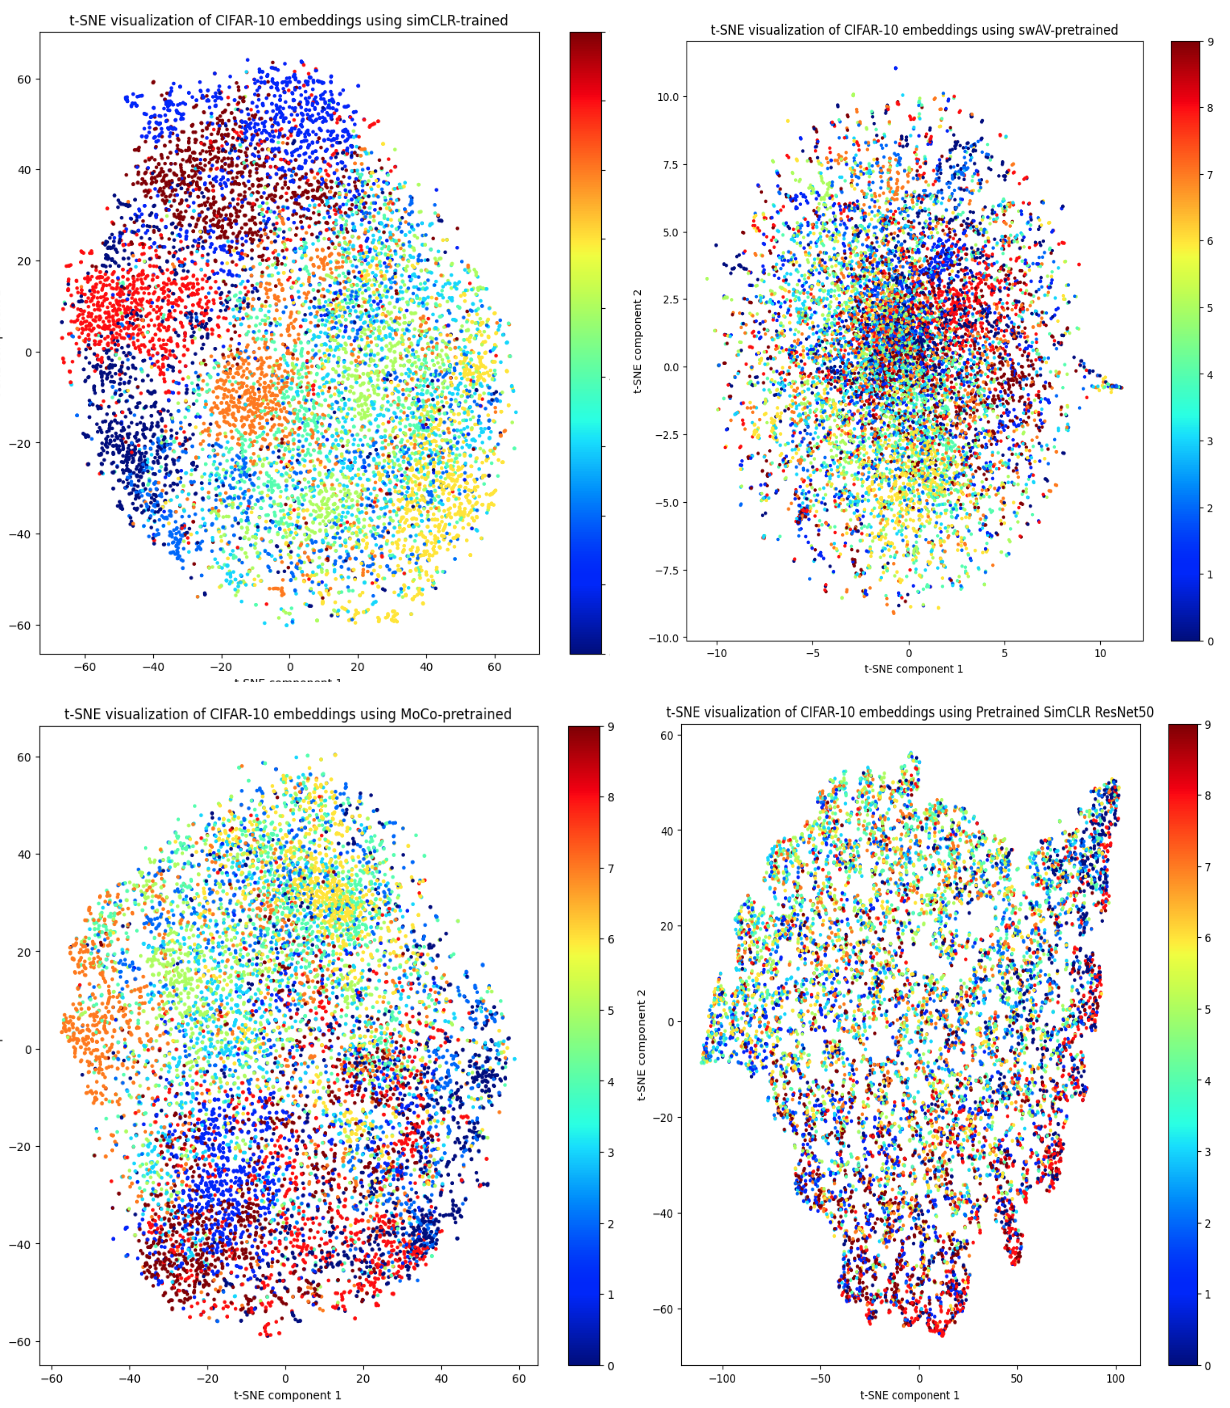
\includegraphics[width=\textwidth]{images/t-SNE-plots.png}
    \caption{t-SNE visualizations of CIFAR-10 test set embeddings from various contrastive models. SimCLR was trained on CIFAR-10, while SwAV, MoCo, and SimCLR ResNet-50 were pretrained on ImageNet. Each point is colored by the ground-truth label. Clearer clustering in the SimCLR-CIFAR10 plot highlights the importance of domain-specific training for representation quality.}
    \label{fig:tsne_plots}
\end{figure*}

\subsection{Visualizing Embedding Spaces of Contrastive Learning Models via t-SNE [\ref{fig:tsne_plots}]}
To understand and compare the semantic quality of embeddings learned by different contrastive learning models, we performed a t-SNE visualization experiment using the CIFAR-10 test set. The goal was to evaluate how well these self-supervised models encode class-discriminative features, even in the absence of labels during training. 

The methodology for the experiment is as follows:
\begin{itemize}

\item Embedding Extraction: For each model, embeddings were extracted from the penultimate layer (or projection head output).
\item Dimensionality Reduction: 2D t-SNE applied on the extracted embeddings.
\item Color Encoding: Each point is colored by its ground-truth class label to assess class-wise separation.
\end{itemize}


The SimCLR model trained on CIFAR-10 produced well-separated clusters, indicating strong alignment between learned representations and ground-truth classes. This suggests that task-specific self-supervised training leads to highly disentangled embeddings. In contrast, the SwAV and MoCo models, both pretrained on ImageNet, showed overlapping and less distinct clusters, with SwAV appearing especially entangled near the center. MoCo demonstrated slightly better class separation, but the embeddings remained noisy and diffuse. The pretrained SimCLR ResNet-50 model showed a distinct spatial structure, but without clear clustering, highlighting that even with the same learning objective, domain mismatch and architecture depth can reduce embedding utility.


\subsection{Evaluating Invariance of Saliency in Self-Supervised Models Using RELAX}

To probe the invariance and stability of self-supervised contrastive models in identifying semantically important regions of an image, we conducted an experiment using RELAX, a recently proposed explainability method for SSL. RELAX generates pixel-level importance masks that highlight the regions most influential to the learned embeddings. Our goal was to test whether these models focus on consistent regions in both original and augmented versions of an image, a core assumption in contrastive learning. This experiment provides insight into whether self-supervised models maintain semantic focus under augmentations. A high degree of alignment would support the claim that these models learn transformation-invariant features, while discrepancies would point to limits in the robustness of their learned representations. 

Methodology for the experiment is as follows:
\begin{itemize}
\item For an image I, compute the RELAX importance mask M\_orig.
\item Apply an augmentation A to obtain I\_aug = A(I).
\item compute RELAX mask M\_aug on I\_aug.
\item Apply the inverse transformation $A^{-1}$ to M\_aug → M\_aug\_inv, aligning it back to the original image space.
\item Compare M\_orig and M\_aug\_inv both:
\begin{itemize}
    \item Visually (overlay masks).
    \item Quantitatively using Intersection-over-Union (IoU):
Threshold each mask using its mean importance value.
Convert to binary mask (1 for pixels > threshold, else 0).
\[
\text{IoU} = \frac{|M_{\text{orig}} \cap M_{\text{aug\_inv}}|}{|M_{\text{orig}} \cup M_{\text{aug\_inv}}|}
\]
\end{itemize}
\end{itemize}

\begin{table}[htbp]
\centering
\caption{Intersection over Union (IoU) between original and augmented image importance masks for different self-supervised models across four augmentations.}
\label{tab:iou_results}
\begin{tabular}{lcccc}
\toprule
\textbf{Model} & \textbf{HFlip} & \textbf{VFlip} & \textbf{Rotate (15°)} & \textbf{Grayscale} \\
\midrule
SwAV & 0.5721 & 0.4508 & 0.4860 & 0.5229 \\
MoCo & 0.6053 & 0.4519 & 0.6990 & 0.8944 \\
SimCLR & 0.6228 & 0.6415 & 0.6183 & 0.7654 \\
\bottomrule
\end{tabular}
\end{table}

Across the three self-supervised learning models—SwAV [fig \ref{fig:swav_relax}], MoCo [fig \ref{fig:moco_relax}], and SimCLR [fig \ref{fig:simclr_relax}]—the RELAX visualizations reveal distinct levels of spatial invariance to common image augmentations. SwAV consistently highlights the key regions (e.g., the subject’s body and head) across all augmentations, demonstrating strong robustness and low uncertainty, particularly after reversing the transformations. In contrast, MoCo exhibits more scattered and augmentation-sensitive attention, with noticeable shifts in importance maps and higher uncertainty, especially under vertical flips and rotations, suggesting weaker localization stability. SimCLR, trained from scratch on CIFAR-10, falls in between: it maintains relatively coherent attention on primary features like the horse bodies, but displays minor instability under more disruptive transformations. Overall, these results reflect how model architecture, training data, and contrastive strategy influence the consistency of learned representations, with SwAV showing the highest invariance and MoCo the least in these visual assessments.

\subsection{GradCAM Experimentation}
\subsubsection{Approaches to implement Grad-CAM}
We have implemented Grad-CAM from scratch to visualize discriminative regions in CNNs, using intermediate feature maps and gradients from various layers of ResNet architectures. We have also experimented with and taken the results of layer choice on spatial resolution and interpretability.

Since Grad-CAM is traditionally used in supervised settings with class-specific gradients, we adapted it for self-supervised models (e.g. simCLR, MoCo v2, SwAV) by introducing proxy tasks such as similarity-based ranking. We have computed gradients of cosine similarity between embeddings of two images with respect to feature maps of ResNet layers, allowing visualization of what features drive representation closeness.

We have selected a pair of images using the two methods below:
\begin{itemize}
    \item The pair of images is an augmented image of a single image.
    \item The pair of images is different but taken from the same class.
\end{itemize}

With the above pair of images, we calculated the cosine similarity and used Grad-CAM to interpret which regions contributed most to high- or low-similarity scores. We have also applied Grad-CAM to a wide range of models, including ResNet50 and its variants.

An experiment has also been conducted to verify and visualize the features that the model has learned, as shown in Figure \ref{fig:gc_plots}.
\begin{figure}[h]
    \centering
    \begin{subfigure}{\linewidth}
        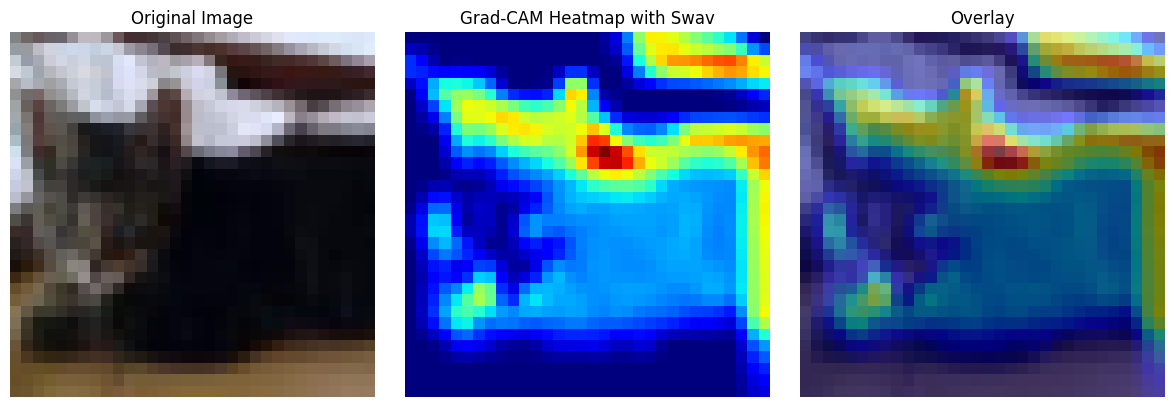
\includegraphics[width=\linewidth]{images/gc1.png}
        \caption{Heatmap augmentation with SwAW}
        \label{fig:gc1}
    \end{subfigure}\vspace{10pt}
    \begin{subfigure}{\linewidth}
        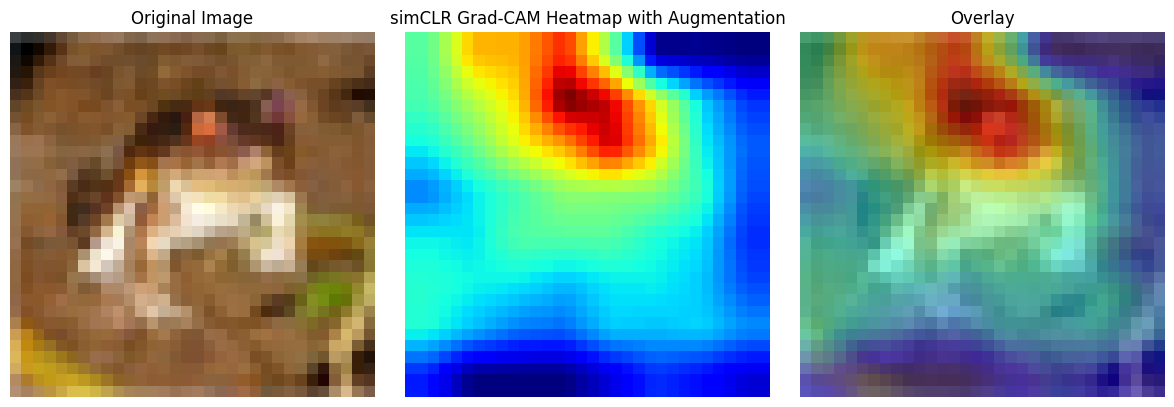
\includegraphics[width=\linewidth]{images/gc2.png}
        \caption{Heatmap augmentation with simCLR}
        \label{fig:gc2}
    \end{subfigure}\vspace{10pt}
    \begin{subfigure}{\linewidth}
        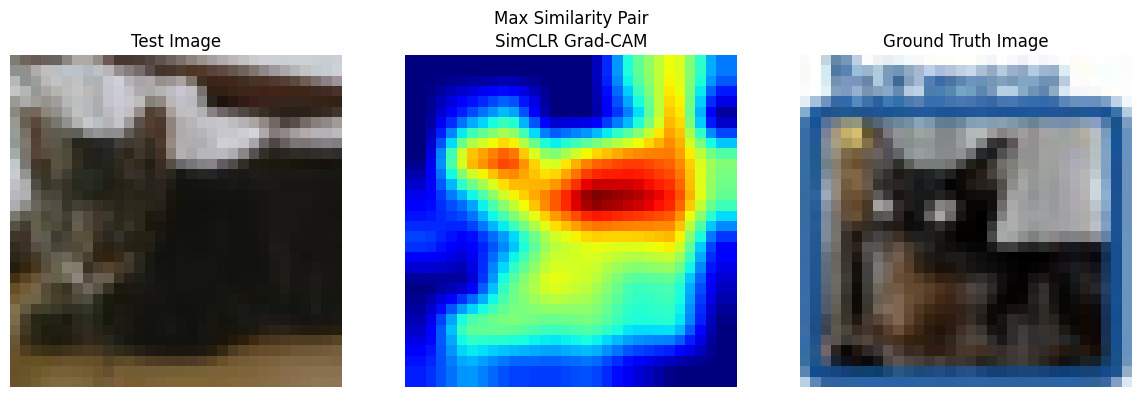
\includegraphics[width=\linewidth]{images/gc3.jpeg}
        \caption{Max similarity pair} 
        \label{fig:gc3}
    \end{subfigure}\vspace{10pt}
    \begin{subfigure}{\linewidth}
        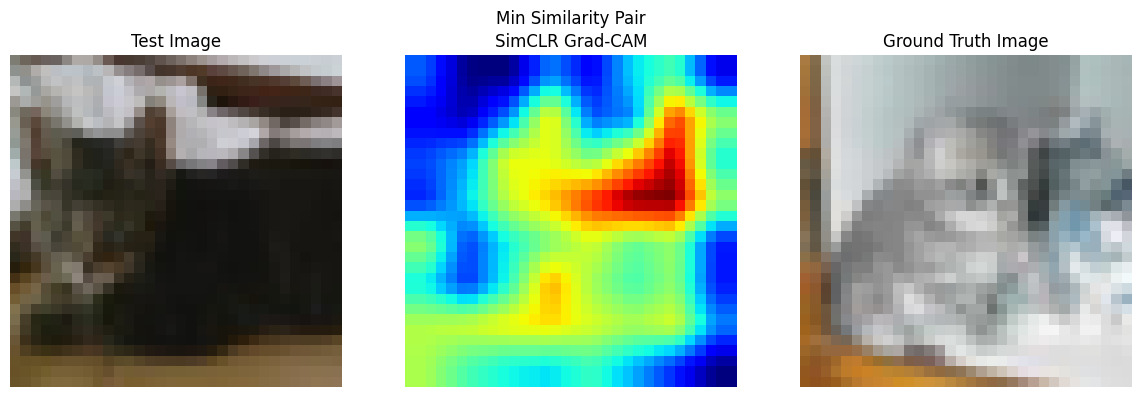
\includegraphics[width=\linewidth]{images/gc4.jpeg}
        \caption{Min simlarity pair }
        \label{fig:gc4}
    \end{subfigure}\vspace{10pt}
    \begin{subfigure}{\linewidth}
        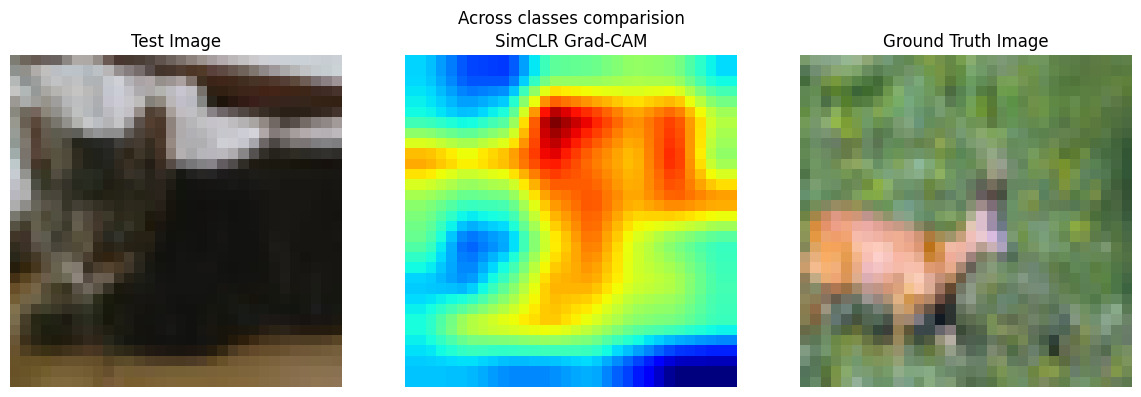
\includegraphics[width=\linewidth]{images/gc5.jpeg}
        \caption{Across class comparison}
        \label{fig:gc5}
    \end{subfigure}
    \caption{Interpretability experiments using GradCAM}
    \label{fig:gc_plots}
\end{figure}

\subsubsection{Interpretability of Learned Features:}
\begin{itemize}
    \item For high similarity pairs, Grad-CAM typically highlights overlapping regions (e.g., face patterns and body of the cat), suggesting the model has learned to focus on semantically meaningful features.
    \item For low similarity pairs, Grad-CAM may either highlight different regions (e.g., one image shows the head of a cat, another its tail) or non-object areas—indicating divergence in learned attention.
\end{itemize}


\subsection{Perceptual Component Explainability}
We began by replicating the original RELAX and modifications mentioned in \cite{yarici2024explaining} for the experimental setup, where the importance of three core perceptual components: color, shape, and texture, was evaluated using attribution-based explanations and frequency-filtered image variants.
This served as a baseline for assessing how different visual properties contribute to the model’s prediction.

\begin{figure}[htbp]
    \centering
    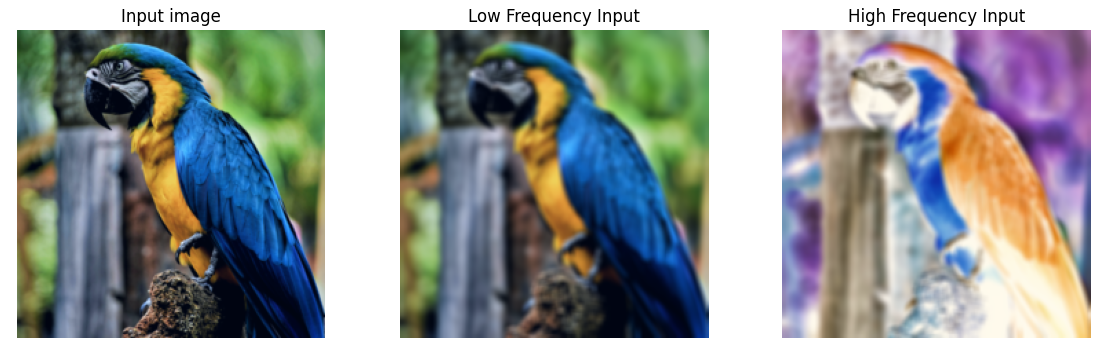
\includegraphics[width=\linewidth]{images/Low-Pass and High-Pass Filtered.png}
    \caption{Input image alongside its low-pass and high-pass filtered versions to isolate frequency components. These versions are used to evaluate the model's reliance on low- and high-frequency visual information.}
    \label{fig:freq_components}
\end{figure}

Following the methodology outlined in \cite{yarici2024explaining}, we extended this analysis to incorporate additional perceptual factors: brightness, depth, and sharpness. Also, as each component uses a sort of filter to get the importance relating to that component, we also tried using a low-pass gaussian filter and a similar high-pass filter. 

For each new perceptual component, we implemented the corresponding transformation pipelines:
\begin{itemize}
    \item \textbf{Brightness}: To evaluate the importance of brightness in the input image, we use the same technique used for color i.e. we replace the masked part by a less brightened version of that part. To get this change of brightness, we first convert the RGB image to LAB [lightness, A (red-green), and B (yellow-blue)], decrement the lightness channel, and then convert the modified image back to RGB.
    \item \textbf{Depth}: We used a MiDas \cite{ranftl2020towards} depth estimation model that computes relative inverse depth from a single image. It has been trained on 10 distinct datasets using multiobjective optimization to ensure high quality on a wide range of inputs. Using this depth map we calculate the importance in a similar manner to the shape and texture.
    \item \textbf{Sharpness}: Sharpness was enhanced by using a Laplacian sharpening kernel, and the importance of sharp regions was determined by the difference between the sharpened image and the input. This approach again parallels the methods used for shape and texture.
\end{itemize}

\begin{figure}[h]
    \centering
    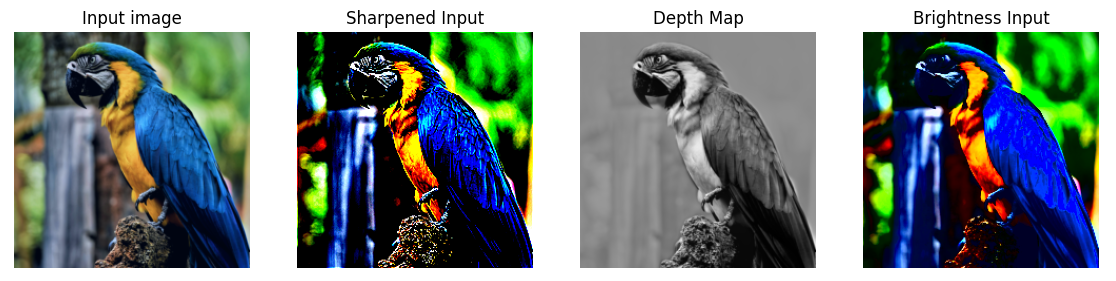
\includegraphics[width=\linewidth]{images/Sharpened, Depth and Brightened Maps.png}
    \caption{Input image, sharpened version, estimated depth map, and brightened image. These perceptual transformations are used to assess sensitivity of models to brightness, depth cues, and sharpness.}
    \label{fig:perceptual_variants}
\end{figure}

In case of perceptual concepts like color, we get the importance maps by replacing the masked area with the same area deprived of that concept. Thus, for perceptual concepts like sharpness and brightness, we replace the mask with a less brightened and sharpened part. In case of perceptual concepts like shapes and textures, we directly use the masks on edge maps,etc. So, similarly in the case of depth, we use the masks directly on the depth map obtained from the model. These images can be seen in Figure \ref{fig:perceptual_variants}.

We can see the results for this experiment in figures \ref{fig:relax_perceptual_maps} and \ref{fig:relax_extended_components}. In general, considering models, the MoCo model (momentum contrast) performs visually better by mainly marking some part of the parrot as important in different importance maps. MoCo also remained the most invariant to these important maps, only showing a spread-out important region for the high frequency filtered map.

Considering the importance maps, the depth map visually looks the best as the background is masked in its doing. The sharpness maps cover most of the parrot body for all the models.

\subsection{SimClr}
We used SimClr as a feature extractor, used same architecture as in \cite{chen2020simple} with a ResNet-18 backbone, and a linear layer on top of the ResNet-18 features. We train the model on CIFAR-10 dataset.

For data augmentation, following techniques are used:
\begin{itemize}
    \item \texttt{Color Jitter}: [0.8, 0.8, 0.8, 0.2] for brightness, contrast, saturation, and hue respectively, is applied to the input image with a probability of 0.8.
    \item \texttt{Random Resized Crop}: Randomly crop the input image and resize it to a given size of 32x32.
    \item \texttt{Random Horizontal Flip}: Randomly flip the input image horizontally with a probability of 0.5.
    \item \texttt{Gaussian Blur}: Apply Gaussian blur to the input image with a kernel size of 0.1*size of the input image, i.e., 3x3 kernel for 32x32 image.
\end{itemize}
Two views are created for each image using the above data augmentation techniques. They are passed through the feature extractor, and loss is minimized.
Below given are the parameters used for training the model:
\begin{itemize}
    \item Epochs: 1000
    \item Batch Size: 256
    \item Learning Rate: 3e-4
    \item Weight Decay: 1e-4
    \item Optimizer: Adam with $\beta_1=0.9$, $\beta_2=0.999$
    \item Scheduler: Cosine Annealing LR Scheduler  
\end{itemize}
Figure \ref{fig:loss_accuracy} shows the training loss and accuracy of the model, in which we achieved an accuracy of 82.8125\%.
\begin{figure}[h]
    \centering
    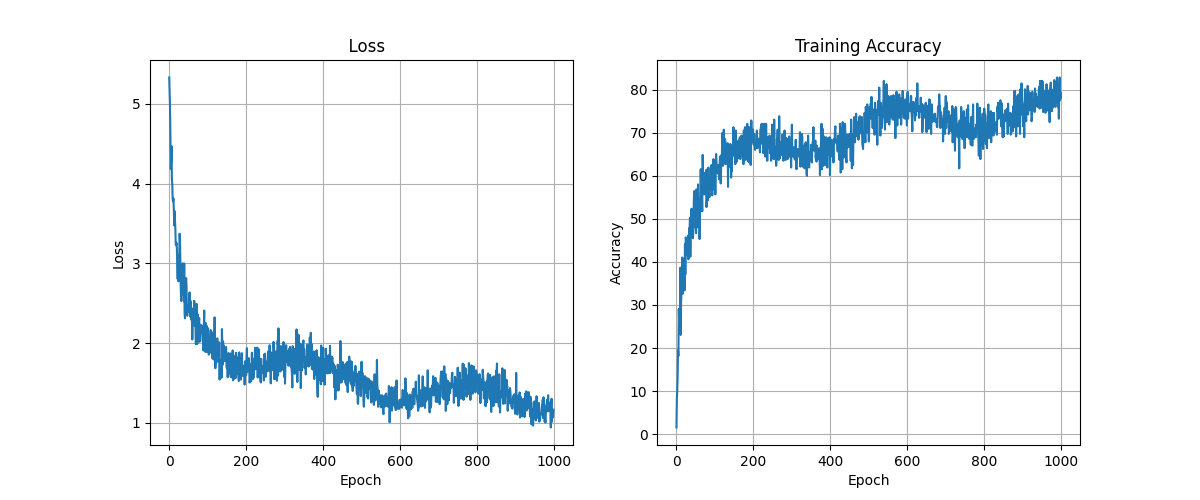
\includegraphics[width=1.0\linewidth]{images/loss_accuracy.png}
    \caption{Loss and Accuracy plot for SimClr}
    \label{fig:loss_accuracy}
\end{figure}

\subsection{Relax}
Our SimCLR trained model is used as a feature extractor for the RELAX\cite{wickstrom2023relax} model. Masks are generated for the input image and simlarity is found between the masked image and the original image. Importance and uncertainty are calculated for each pixel in the image using simlarity scores.

Figure \ref{fig:result1}, \ref{fig:result2}, and \ref{fig:result3} show the RELAX explanation and uncertainty on CIFAR-10 dataset. In the figure \ref{fig:result2}, model is able to give importance to the aeroplane in the image and uncertainty is high in the background. In the figure \ref{fig:result3}, model is able to give importance to the bird in the image and uncertainty is high in the background. This shows that RELAX model is able to give importance to the object in the image and uncertainty in the background. 
\begin{figure}[h]
    \centering
    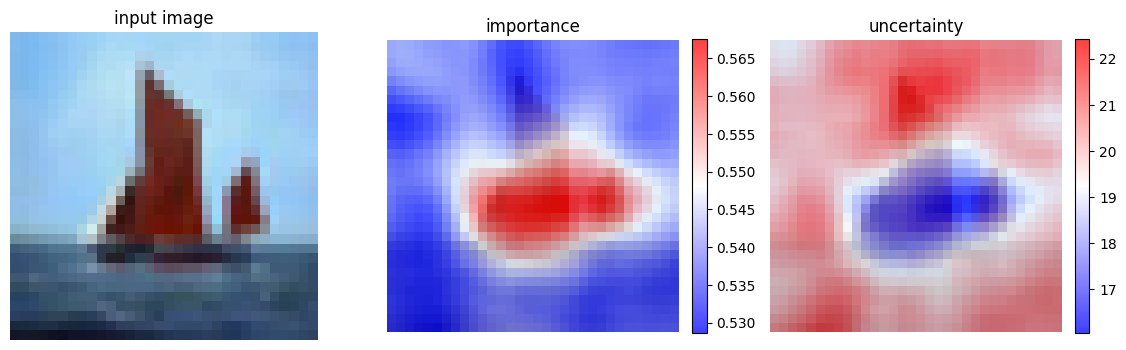
\includegraphics[width=1.0\linewidth]{images/Result1.png}
    \caption{RELAX explanation and uncertanity on CIFAR-10 dataset}
    \label{fig:result1}
\end{figure}
\begin{figure}[h]
    \centering
    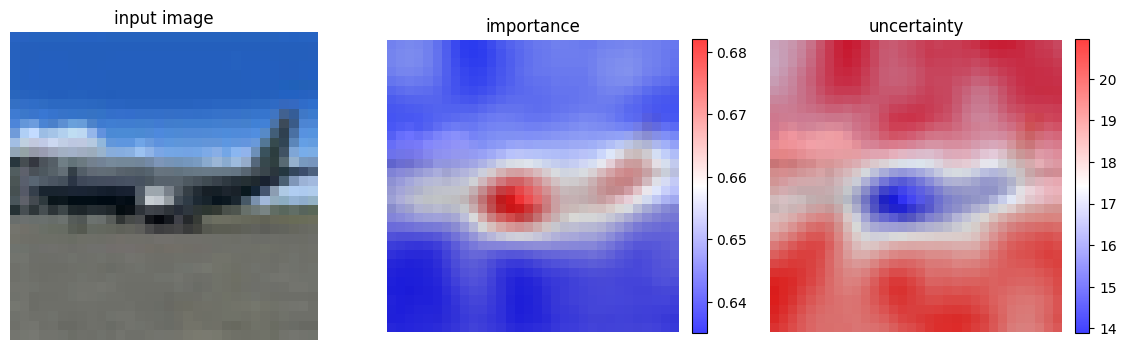
\includegraphics[width=1.0\linewidth]{images/Result2.png}
    \caption{RELAX explanation and uncertanity on CIFAR-10 dataset}
    \label{fig:result2}
\end{figure}
\begin{figure}[h]
    \centering
    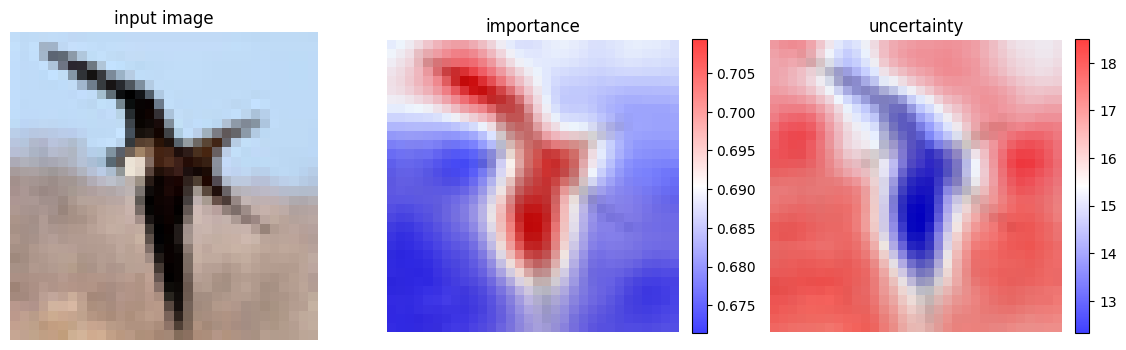
\includegraphics[width=1.0\linewidth]{images/Result3.png}
    \caption{RELAX explanation and uncertanity on CIFAR-10 dataset}
    \label{fig:result3}
\end{figure}

